
%%%%%%%%%%%%%%%%%%%%%%%%%%%%%%%%%%%%%%%%%%%%%%%%%%
\section{Data Quality}
%%%%%%%%%%%%%%%%%%%%%%%%%%%%%%%%%%%%%%%%%%%%%%%%%%
\subsection{Collected Data}

Table~\ref{Table:Data} shows list of the collected data while Oct/2010 Run.
800 MeV/$c$ pion is expected to pass-through the detector as MIP,
and have uniform energy deposition to all the TPC channels.
So this data set is very useful for calibrating the detector response (See section xxx).
800 MeV/$c$ proton stops after ~15 cm of flight distance inside the TPC fiducial volume
with relatively large $dE/dx$. So we use the proton data set for validation of the
detector response at high $dE/dx$ region(See section xxx).
We have collected three different Kaon data by varying thickness of the degrader. 
540, 630, 680 MeV/$c$ are corresponds to the momentum degraded by 
2 lead glass, 1 lead glass + 1 lead block, and 1 lead glass, respectively, 
and such Kaon stops after 10 cm, 50 cm, and 65 cm of flight distance inside TPC fiducial volume.

Figure~\ref{Fig:Textbook} shows an 2D display of typical event 
taken with 800 MeV/$c$ electron trigger.
Horizontal axis corresponds to TPC channel number 
and zero means most upper stream strip. 
Since strip pitch is 1 cm, this is equivalent to
distance from beam injection point in cm.
Vertical axis corresponds to electron drift time in $\mu$s
and t=0 means trigger timing. In this TPC, anode and cathode is
located at top and bottom of the detector, respectively,
t=0 means energy deposition at anode and longer drift time 
means energy deposition in lower height.
With 200 V/cm of electric field, drift velocity is about 0.8 m/ms.
So drift of full detector (40 cm) takes 500 $\mu$s.
Color strength of the plot corresponds to the TPC signal pulse height
in ADC counts which is roughly proportional to $dE/dx$ of the track.
In this event, triggered electron can be clearly seen center of the detector
as an electromagnetic shower while there are two other particles 
accidentally overlapped with the triggered electron. 
Track at t=100 $\mu$s is considered as
a proton which stops after 15 cm of flight distance and 
has large $dE/dx$ around the stopped point.
Track at t=400 $\mu$s is considered as
a pion which passes-through the detector and 
has uniform $dE/dx$ over the TPC channels.
This event already gives us some idea for how good 
the particle identification performance of the LArTPC is.

Figure~\ref{Fig:Kmunu} shows a typical $K \to\mu\nu$ like event.
We can clearly identify a kink of the track at 60 cm which is considered
as stopped point of Kaon and it decays to  

Energy deposition of the track is about MIP at the injection point
and gradually increase towards the stopped point at 60 cm.



\begin{table}[h]
\begin{center}
\caption{List of collected data}
\begin{tabular}{l|ll}
  Particle  &Momentum (MeV/$c$) &Number of Events\\
\hline
  Pion      &800                &3,000\\
  Proton    &800                &1,500\\
  Kaon      &540 (2LG)          &7,000\\
  Kaon      &630 (1LG+1LB)      &40,000\\
  Kaon      &680 (1LB)          &35,000\\
  electron  &800                &2,500\\
  electron  &200                &10,000\\
  pion      &200                &10,000\\
\end{tabular}
\label{Table:Data}
\end{center}
\end{table}



\begin{figure}[htbp]
 \begin{center}
  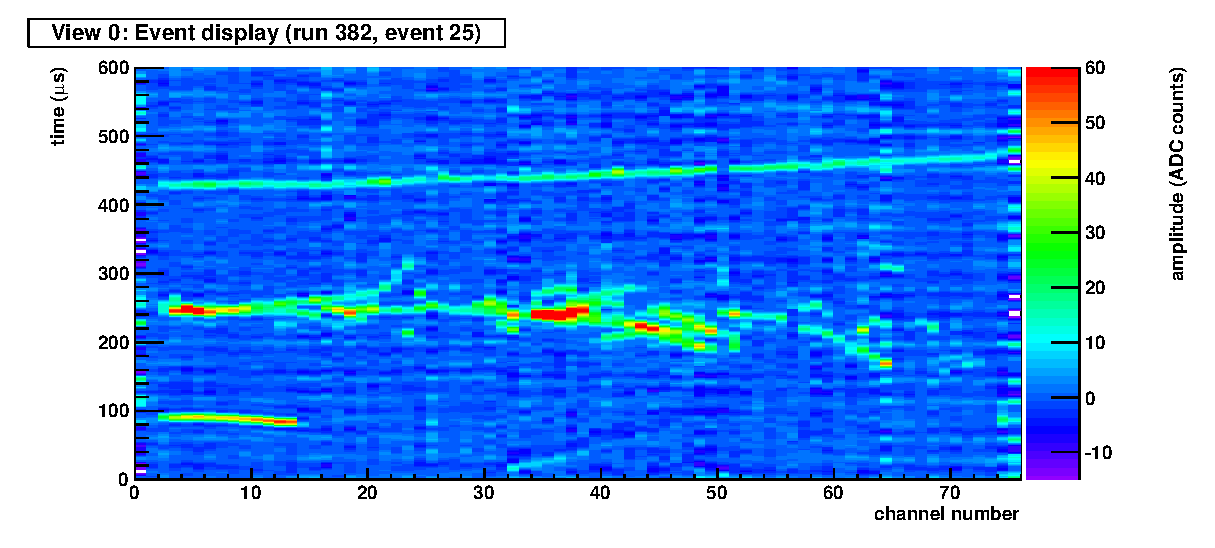
\includegraphics[width=100mm]{fig/Textbook.eps}
 \end{center}
 \caption{Event display of 800 MeV/$c$ electron triggered event.
Accidentally overlapped with a proton and a pion.}
 \label{Fig:Textbook}
\end{figure}

\begin{figure}[htbp]
 \begin{center}
  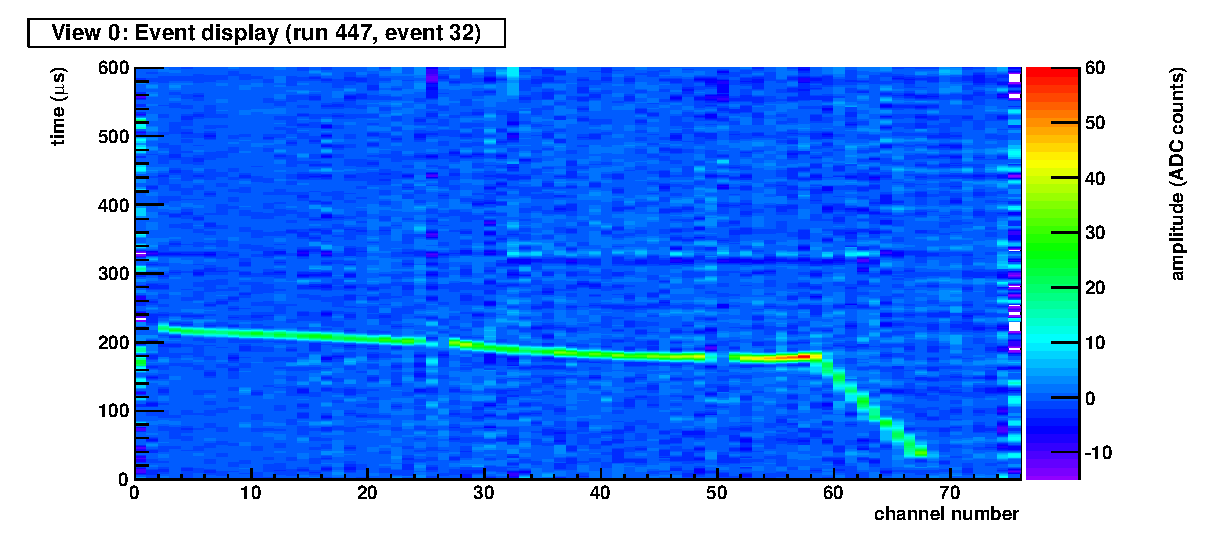
\includegraphics[width=100mm]{fig/Kmunu.eps}
 \end{center}
 \caption{Event display of Kaon 630 MeV/$c$ triggered event}
 \label{Fig:Kmunu}
\end{figure}

%\subsection{Beam Quality}
\subsection{Beam Quality(Purity)}

We have several beam counters to indentify beam particles event by event(see Fig\ref{fig:Beamline}).Using this when taking data, we can get data of interest selectively.The following describe how to identify beam particles with the typical data including $K^{+}$, $\pi~{+}$, $e^{+}$, $p$ events, which have the momentum adjusted $\sim$800MeV/c.\\

\begin{figure}[htbp]
  \centering
  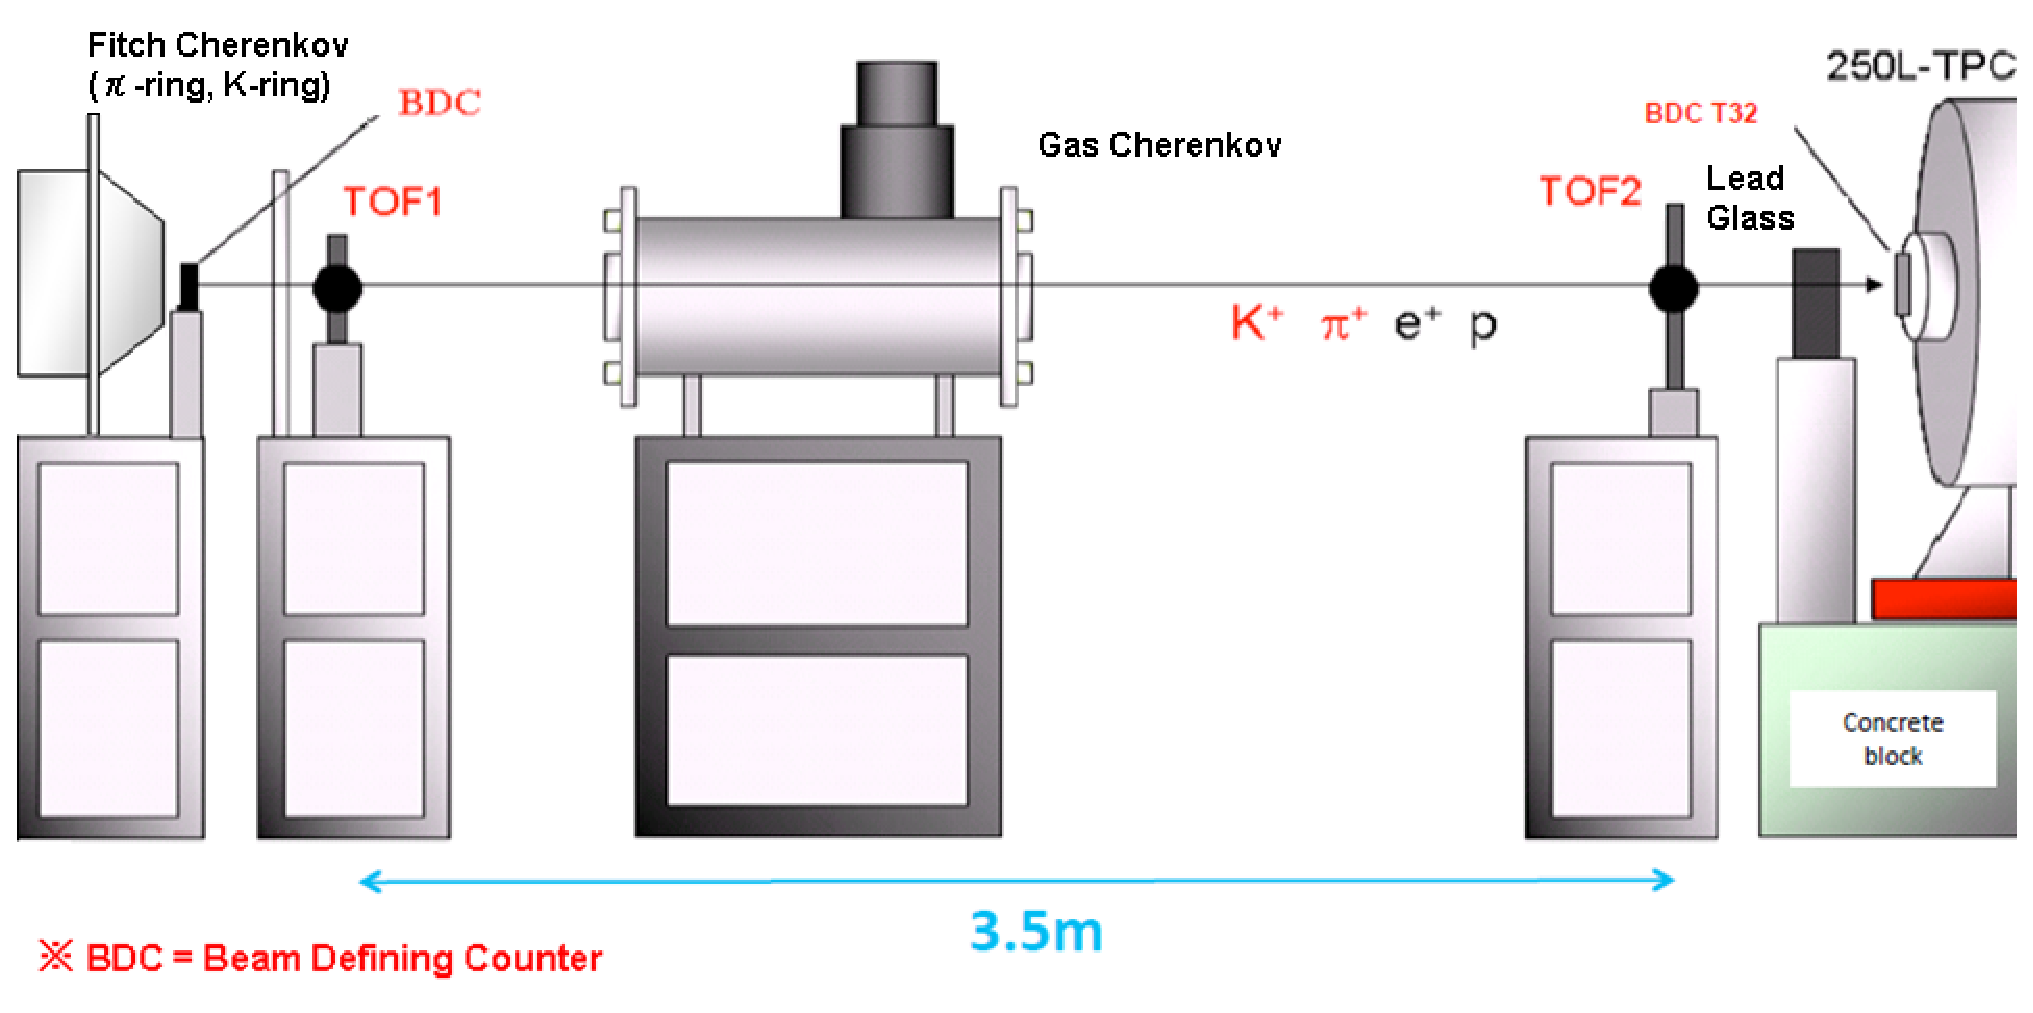
\includegraphics[width=10cm,clip]{fig/Beamline.eps}
  \caption{Instruments on K1.1BR Beam Line}
  \label{fig:Beamline}
\end{figure}

Leaded particles to K1.1BR beamline pass the Fitch Cheernkov Counter at first.
Fitch Cherenkov Counter can select particles with diffrerences of angle of cherenkov light which they radiate.
Fifure\ref{fig:FC_KPI} shows the respose of the Fitch Cherenkov Counter.
The horizontal axis shows the total amount of PMT signal where cherenkov light of 800MeV/c $\pi$ can be detected.
The vertical axis shows that of 800MeV/c $K$.
Signals are distinctly seperated to three cluster and can be categolized as following.\\

\begin{enumerate}
\item FC Signal($\pi$)$<$1450 \& FC Signal($K$)$>$2000 \\
\item FC Signal($\pi$)$<$1450 \& FC Signal($K$)$<$2000 \\
\item FC Signal($\pi$)$>$1450 \& FC Signal($K$)$<$2000 \\
\end{enumerate}

Appearently, particles within the region 1 are $K^{+}$ candidates.
Particles within region 2 are $p$ candidates because 800MeV/c $p$ is impossible to radiate cherenkov light.
Particles within region 3 are $\pi^{+}$ or $e^{+}$ candidates because their angle of cherenkov light are almost same level.\\

\begin{figure}[htbp]
  \centering
  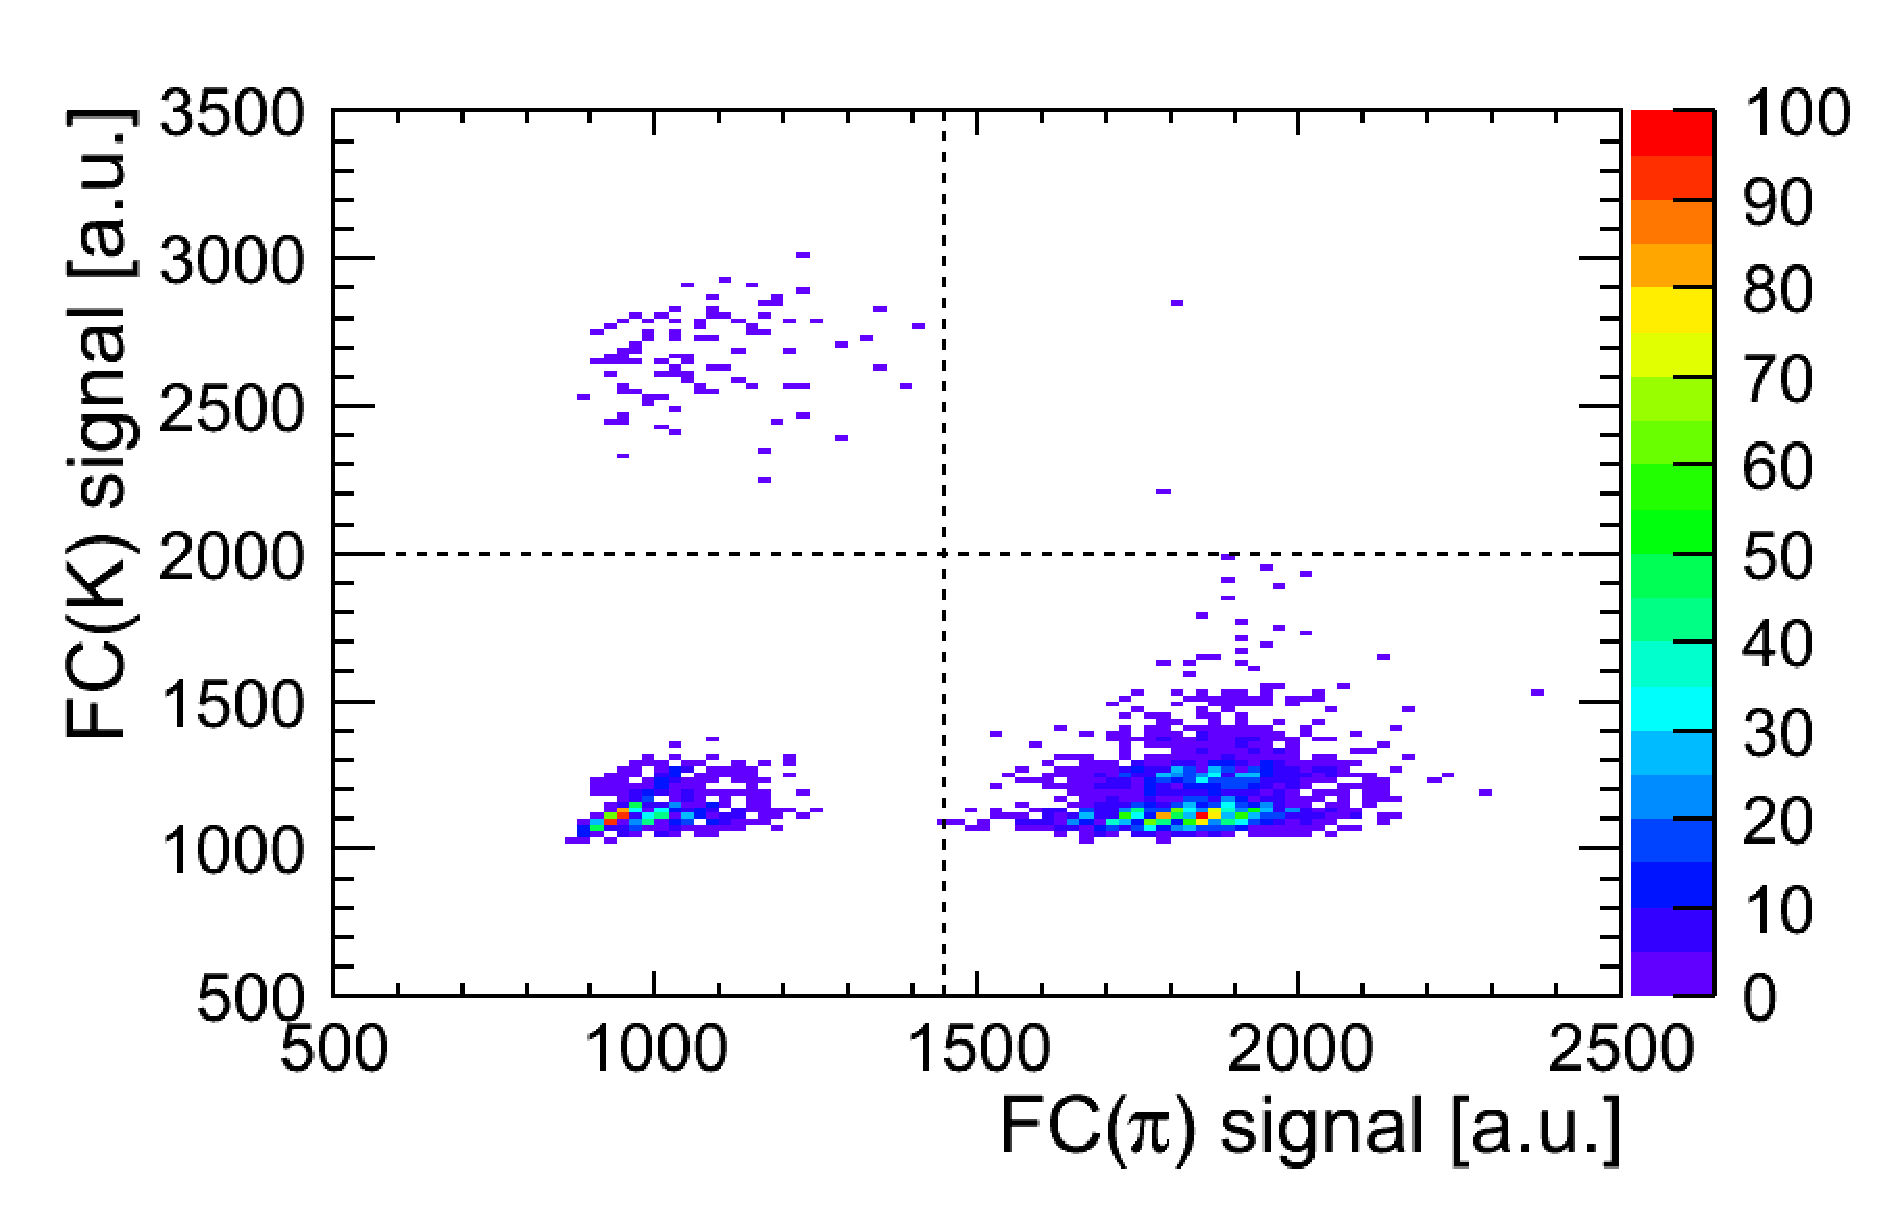
\includegraphics[width=10cm,clip]{fig/FC_KPI.eps}
  \caption{Fitch Cherenkov Counter}
  \label{fig:FC_KPI}
\end{figure}

Gas Cherenkov Counter can select $e^{+}$ from the other particles because only $e~{+}$ can radiate cherenkov light at the refractive index of this gas.
Figure\ref{fig:GC} shows the responce of the Gas Cherenkov Counter.
The horizontal axis shows the PMT signal of the Gas Cherenkov Counter.
The vertical axis shows the number of events.
Fitting the pedestal with gaussian function,
the events larger than the value added $\sim$3.5$\sigma$ to the mean of the pedestal is $e^{+}$ candidates.In this case, GC signal is required more than 104.7 to be $e^{+}$ candidates.\\

\begin{figure}[htbp]
  \centering
  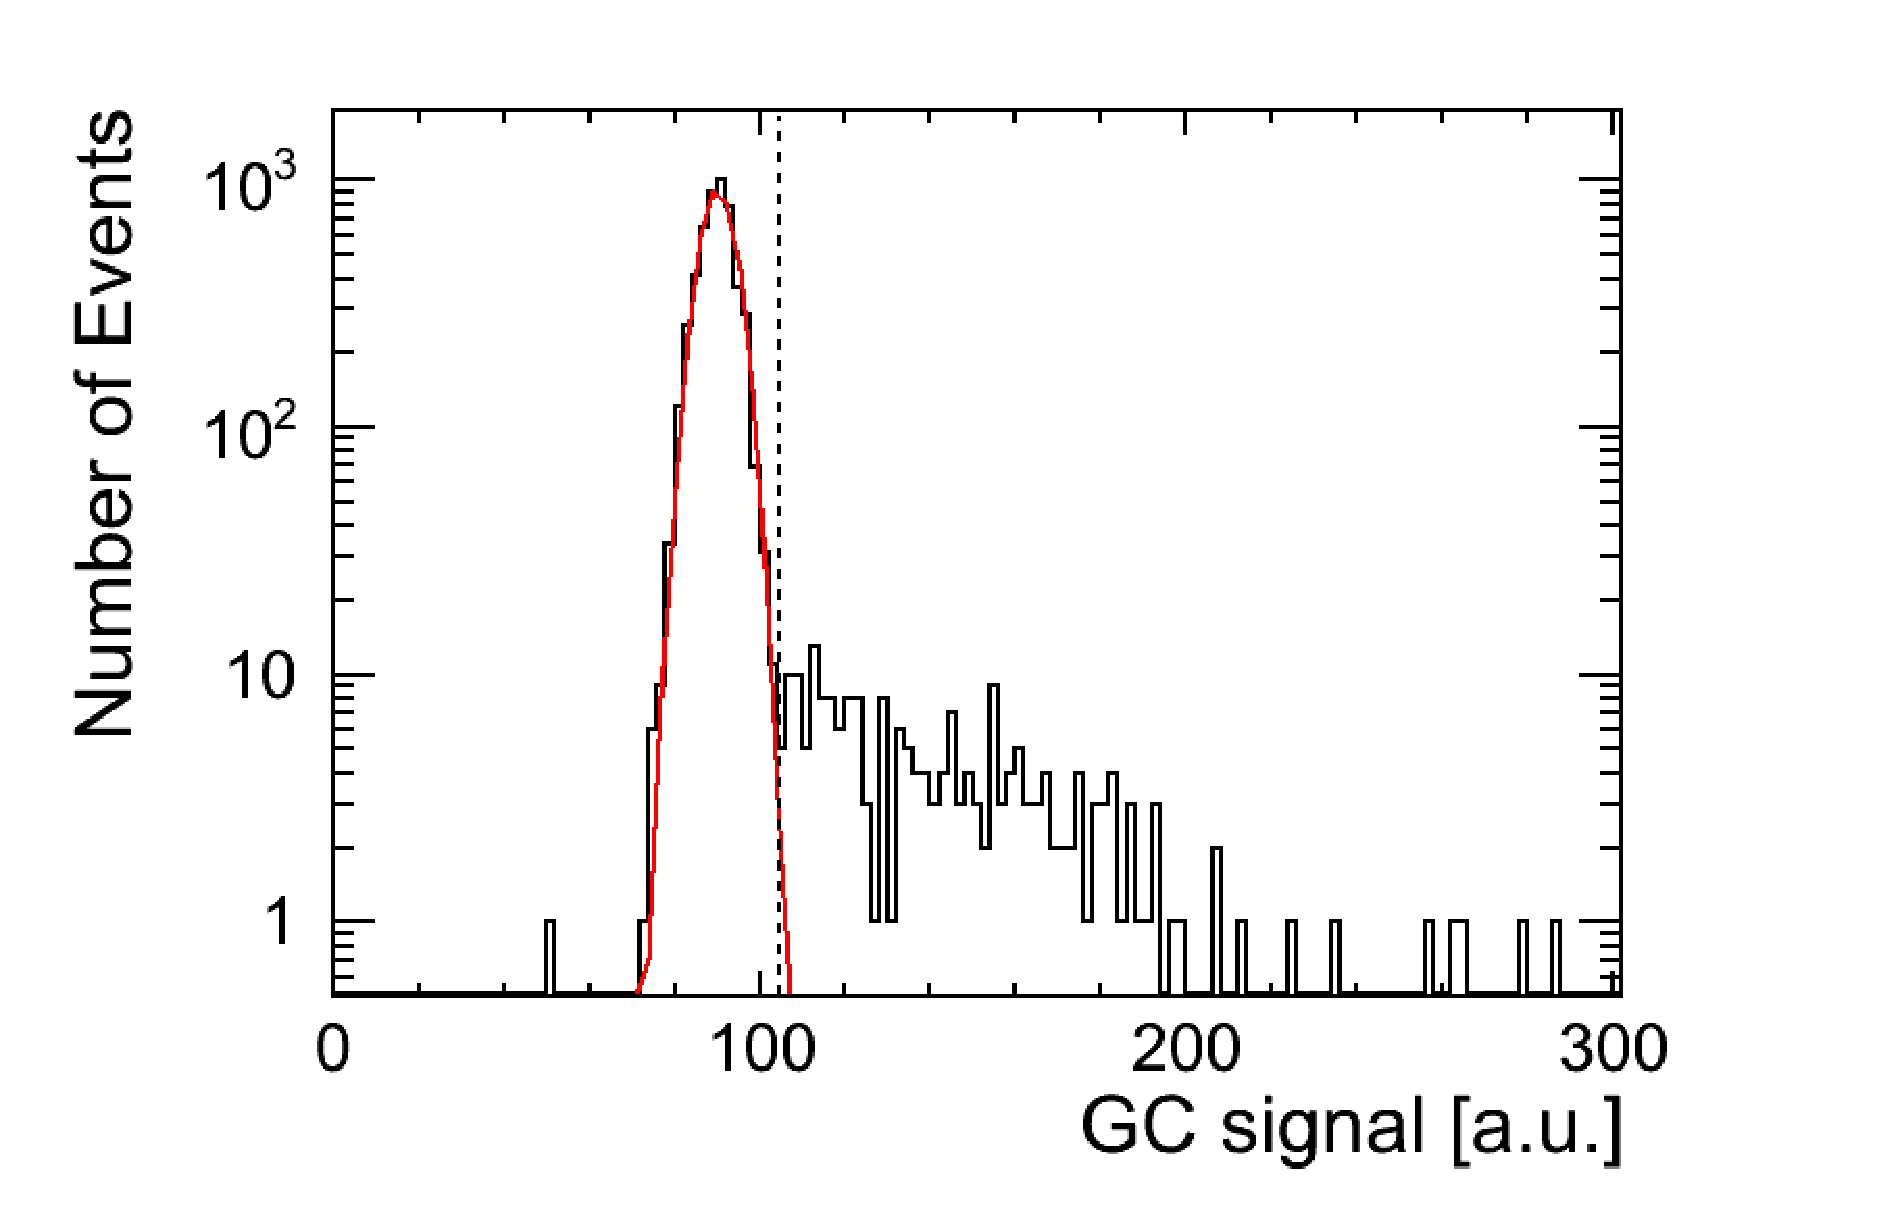
\includegraphics[width=10cm,clip]{fig/GC.eps}
  \caption{Gas Cherenkov Counter}
  \label{fig:GC}
\end{figure}

There are two TOF Counters which has $\sim$200ps resolution 3.5m apart, 
and each particle can be selected with the difference of time of flight between them.
Following table\ref{tb:TOF_expect} is calcurated time of flight when each 800MeV/c particle passes two conters.
As this table shows, $e~{+}$ and $\pi^{+}$ cannot selected because the difference of time of flight is too short for the TOF resolution.\\

\begin{table}
  \centering
  \begin{tabular}[htb]{c|cccc}\hline
    particle & $e^{+}$ & $\pi^{+}$ & $K^{+}$ & $p$ \\ \hline
    Mass(MeV) & 0.511 & 139.57 & 493.68 & 938.27 \\
    Time of Flight($ns$) & 11.67 & 11.84 & 13.71 & 17.98 \\ \hline
  \end{tabular}
  \caption{Time of flight of eash particle}
  \label{tb:TOF_expect}
\end{table}

Figure\ref{fig:TOF} shows responce of the TOF Counters.
The horizontal axis shows the time of flight between TOF1 and TOF2 Counter.
The vertical axis shows the number of events.
Signals have clearly divided three structures.
From table\ref{tb:TOF_expect}, in asending order of time of flight the first structure include $e^{+}$ or $\pi^{+}$ candidates,
and the second struature include $K^{+}$ candidates,
and the third structure include $p$ candidates.
The cut value to separete the first strucuture and the second structure is $\sim$4.5$\sigma$ (in this case, the value is setted 13.15ns), and because the second structure and the third structure is clearly separated, the cut value to select them is setted 16.47ns fully apart from the second structure.\\

\begin{figure}[htbp]
  \centering
  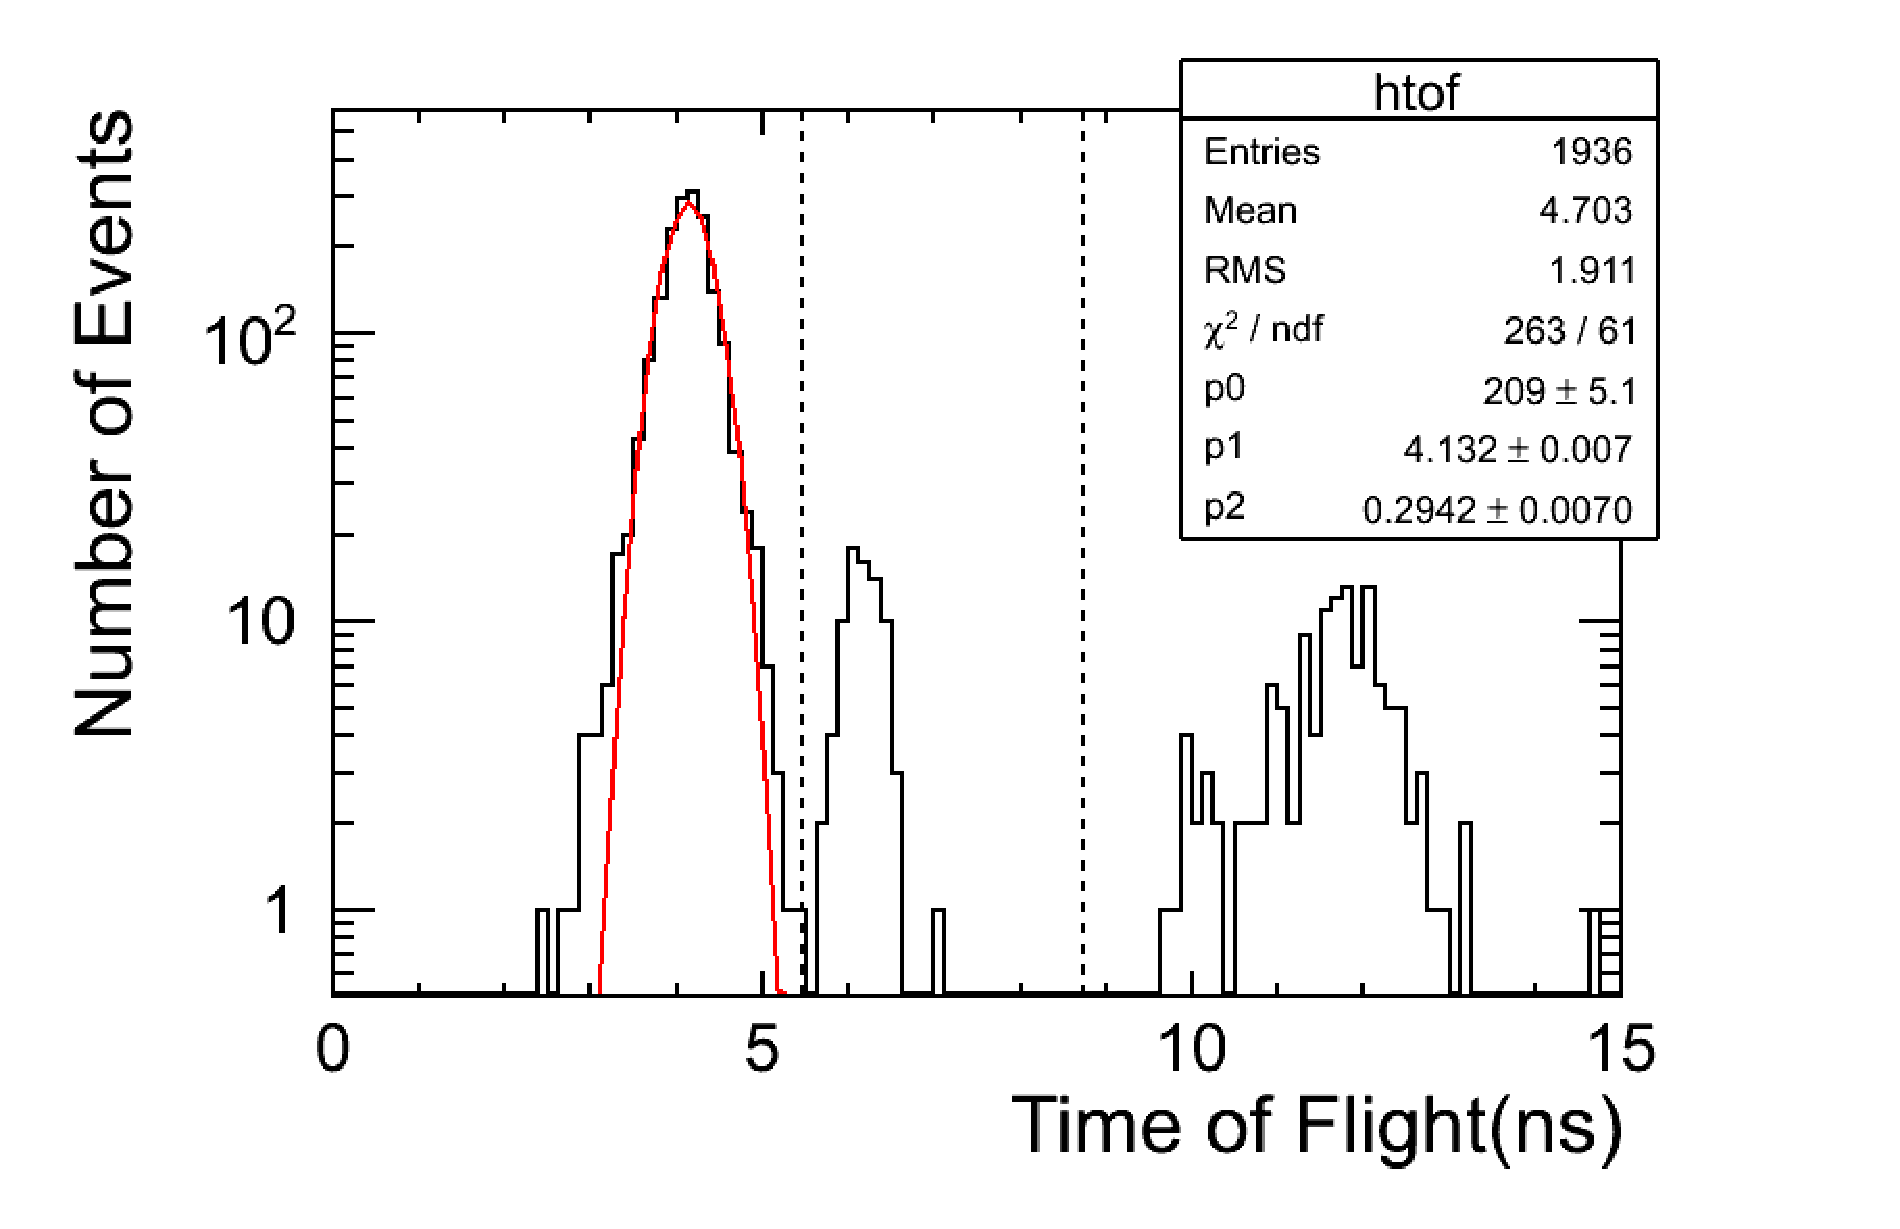
\includegraphics[width=10cm,clip]{fig/TOF.eps}
  \caption{TOF Counter}
  \label{fig:TOF}
\end{figure}

$K^{+}$ can selected very efficiently with Fitch Cherenkov Counter,
so we require the condition FC Signal($K$) is more than 2000
to get the date of $K$ in taking data.
Figure\ref{fig:TOF_cut} shows responce of the TOF Counters before and after above cut.
The histgram which filled with black is what is after cut.
This figure shows we can get high-purity $K^{+}$ samples with this condition.

\begin{figure}[htbp]
  \centering
  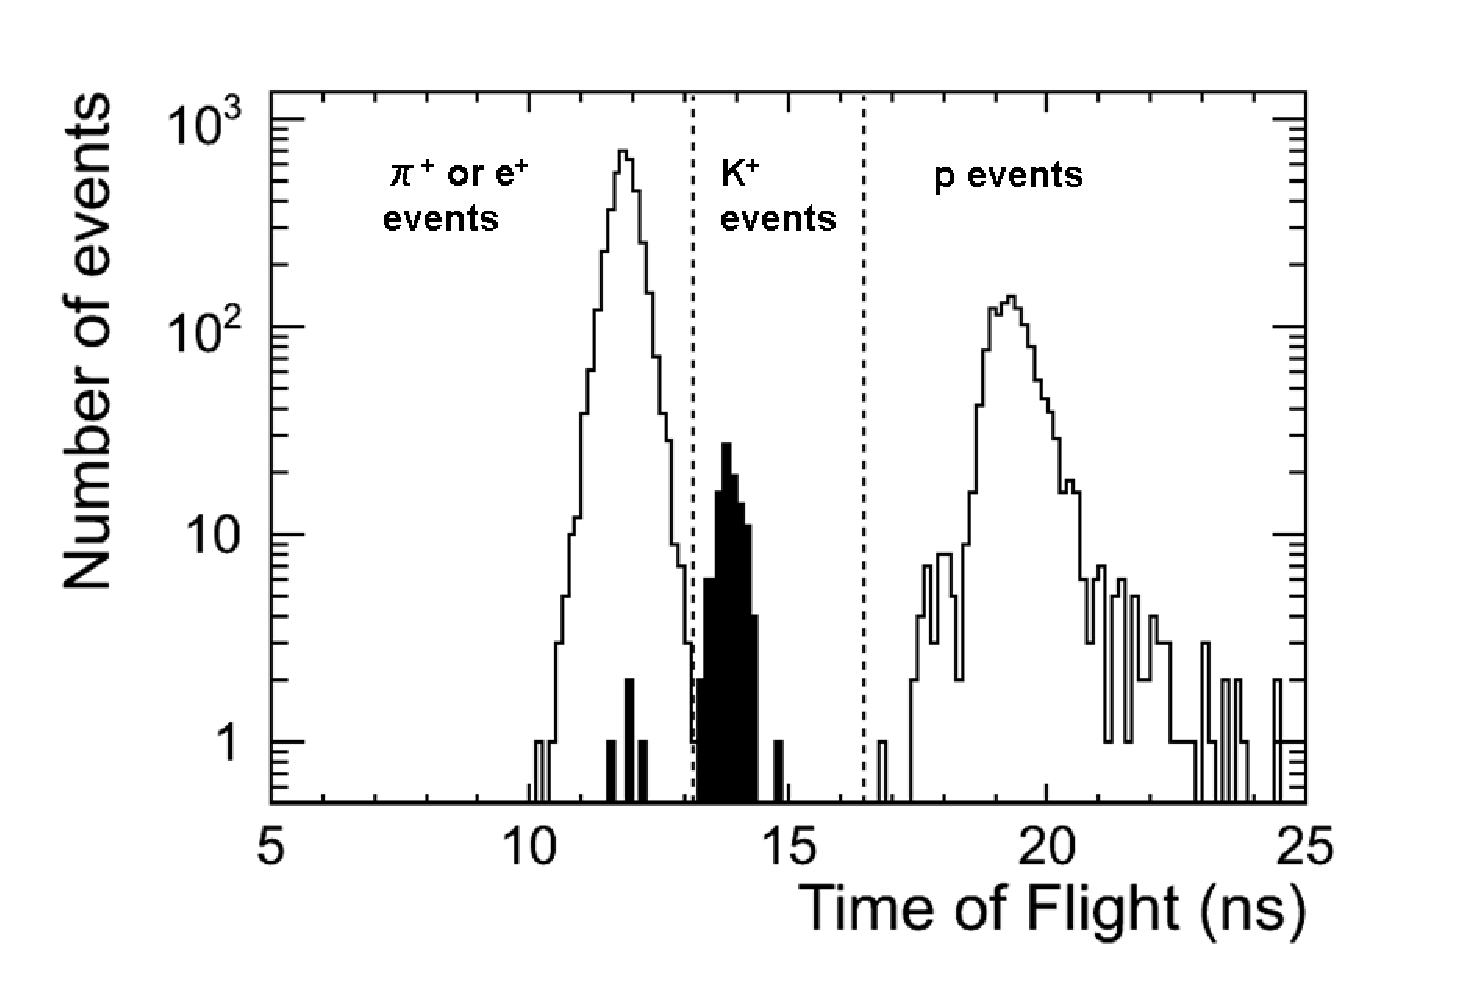
\includegraphics[width=10cm,clip]{fig/TOF_cut.eps}
  \caption{TOF Counter}
  \label{fig:TOF_cut}
\end{figure}

Particles which satisfy all conditions for the same candidate are identified themselves, and the others are defined `uncertain` particles.
Herewith, we can identify beam particles with high purity before injection to 250L detector.
Table\ref{tb:component} shows the beam components of the data used for analysis.\\

\begin{table}
  \centering
  \begin{tabular}[htb]{ccccccc}\hline
    Run Number    & $e^{+}$ & $\pi^{+}$ & $K^{+}$ & $p$   & $uncertain$ & Number of Events \\ \hline
    42            & 68      & 1617      & 27      & 232   & 5           & 1949             \\
    48            & 128     & 1594      & 78      & 126   & 11          & 1937             \\
    49            & 0       & 341       & 0       & 1146  & 12          & 1499             \\
    52            & 0       & 1         & 3126    & 0     & 76          & 3203             \\
    55            & 0       & 6         & 8386    & 0     & 208         & 8600             \\
    59            & 0       & 8         & 5863    & 0     & 119         & 5963             \\
    60            & 0       & 1         & 1870    & 0     & 40          & 1911             \\ \hline
  \end{tabular}
  \label{tb:component}
  \caption{Beam components of data ued for analysis}
\end{table}

Run 52,55,59 and 60 are the data required the condition FC Signal($K$) is more than 2000 in taking data.
As table\ref{tb:component} shows, these data is almost occupied $K^{+}$ events and the ratio is $\sim$98\% on average.

 
%\subsection{Beam Energy, Position}
   \section{Beam Energy, Position}
   \subsection{Beam Energy}
 
   30GeV proton beam hits to target T1 in Hadron hall.
   It generates many particles like kaon, pion, muon, electron, and
   so on.
   We take the particles that has 800MeV/c momentum from this beam by
   using D1 magnet.\\
   \ \ For this analysis, a beam momentum at BDC after passing through the
   K1.1Br beam line is required.
   We estimate a beam momentum using simple MC simulation.
   Figure \ref{K11Br_Beam_line} shows MC simulation's geometory.
   This time, beam line is straight and has no electric and magnetic
   field.
   MC simulation shoot 800MeV/c kaon and pion as pencil beam.

   Figure \ref{k_pi_momentum} shows kaon and pion momentum distribution
   using this MC simulation.
   Actually, kaon momentum distribution peak is adjusted so that kaon
   decay point of MC simulation is consistent with data.
   Section \ref{kaon_energy_section} explains this point.
   And proton momentum is estimated in other way, using TREK detector
   TOF information.
   Section \ref{proton_energy_section} shows proton momentum distribution.

   \subsubsection{Kaon energy}\label{kaon_energy_section}

We adjust momentum peak of figure ?? and set Kaon beam energy  the point that the decay points of Kaon in data and simulation are good agreement. The distribution of decay poins are plotted in Figure\ref{DecayPoint_hough}.
\begin{figure}[!htb]
  \begin{center}
    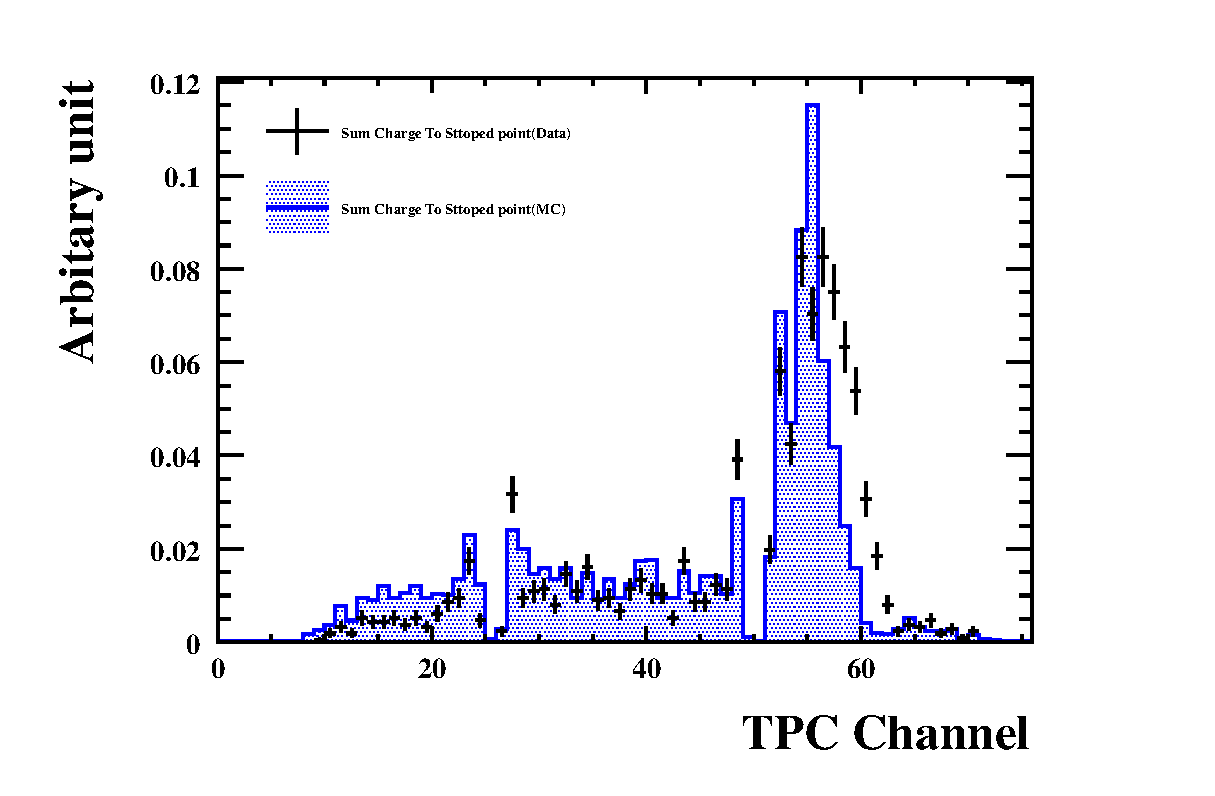
\includegraphics[width=70mm]{fig/cdp_hough.eps}
  \end{center}
  \caption{Decay point distribution of Data and MC}
  \label{DecayPoint_hough}
\end{figure}

   \subsubsection{Proton energy}\label{proton_energy_section}
   asuka




   \subsection{Energy deposition in degrader}
   Because of having high energy, kaon beam from BDC passes through 250LAr TPC.
   So that kaon stops in 250LAr TPC, we put degrader, which reduce
   beam energy, on beam line.
   In this experiment, we used lead glass and lead block as degrader.
   We estimate energy deposition in degrader by using MC simulation.
   Figure \ref{energy_deposition} shows energy deposition in degrader.
   
   \subsection{Beam Position}
   Before taking data, we measured a beam profile on the front of
   250LAr TPC by using plastic scintillation counter.
   Figure \ref{beamprofile_250L} shows beam profile on the front of
   250LAr TPC.

   \begin{figure}[!htb]
    \centering
    \centering
    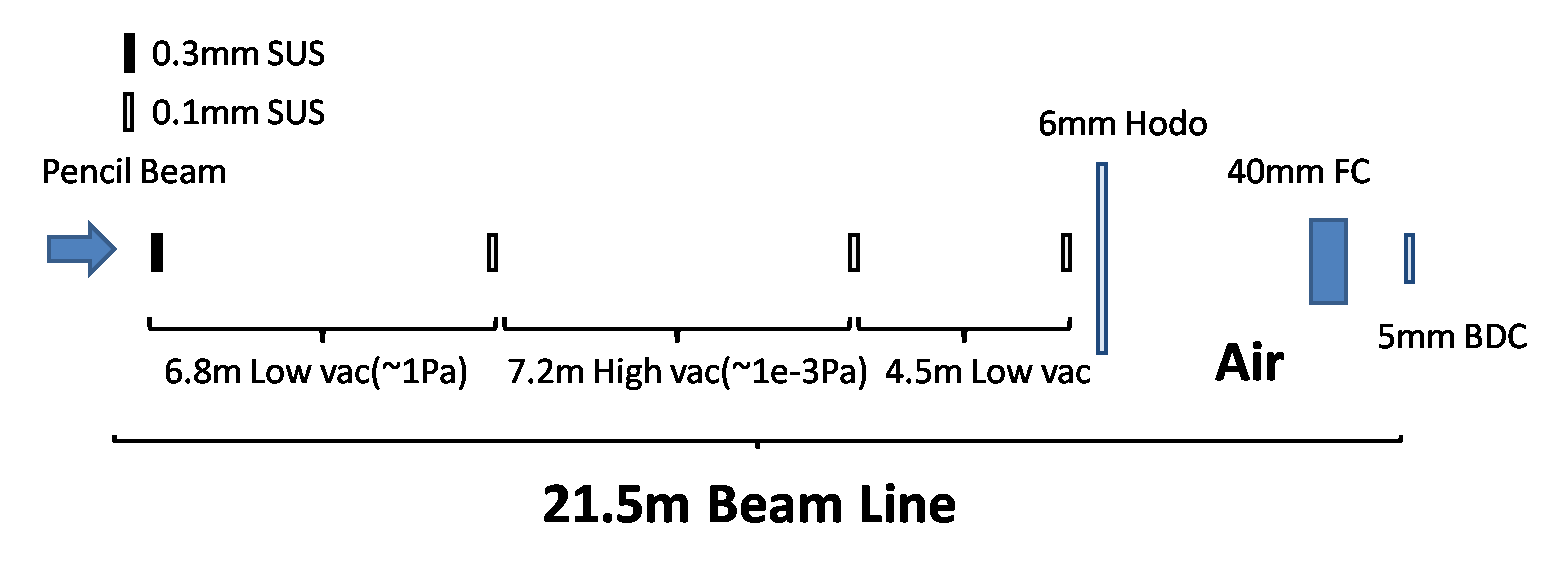
\includegraphics[width=11cm,clip]{./fig/K11Br_beamline_sim.eps}
    \caption{K1.1 Br beamline}
    \label{K11Br_Beam_line}
   \end{figure}



   \begin{figure}[!htb]
    \centering
    \centering
    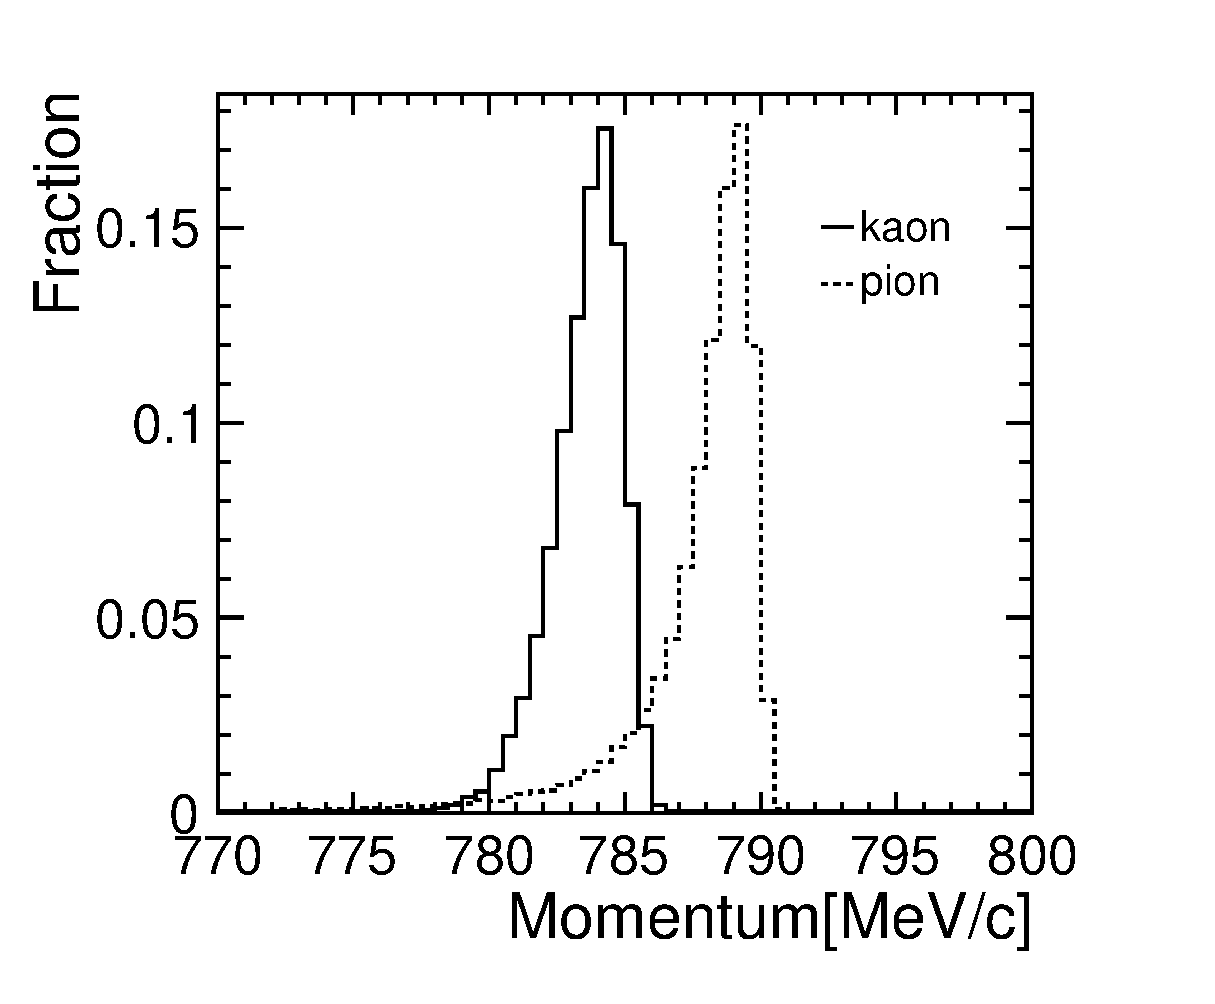
\includegraphics[width=11cm,clip]{./fig/Kaon_pion_momentum_nogrid.eps}
    \caption{kaon and pion momentum distribution at BDC}
    \label{k_pi_momentum}
   \end{figure}


   \begin{figure}[!htb]
    \centering
    \centering
    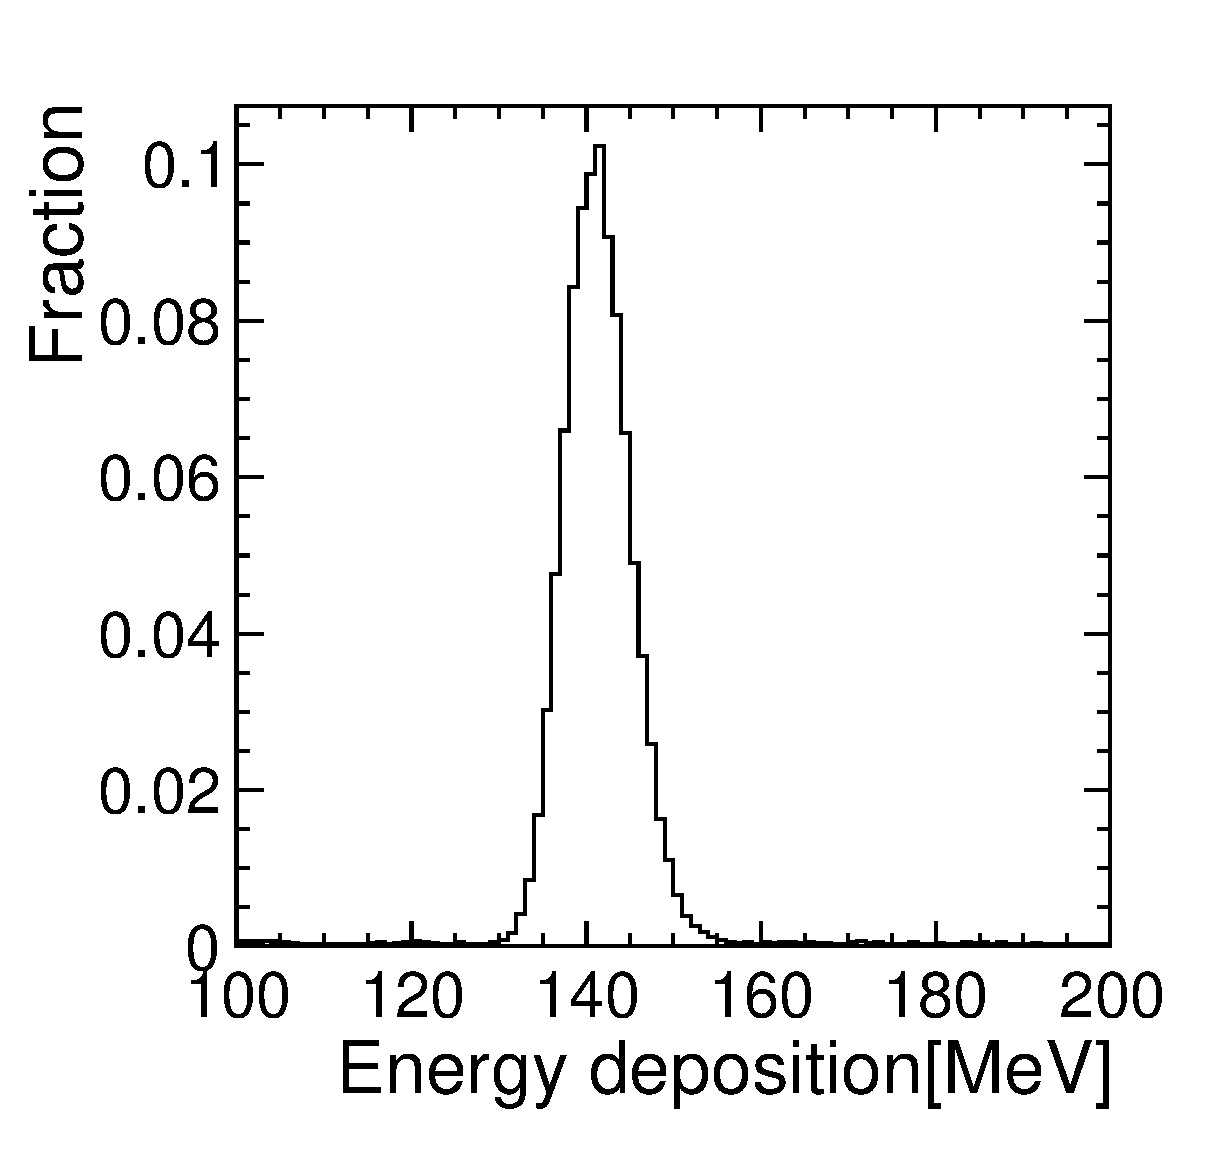
\includegraphics[width=11cm,clip]{./fig/energy_deposition.eps}
    \caption{energy deposition in degrader}
    \label{energy_deposition}
   \end{figure}


   \begin{figure}[!htb]
    \centering
    \centering
    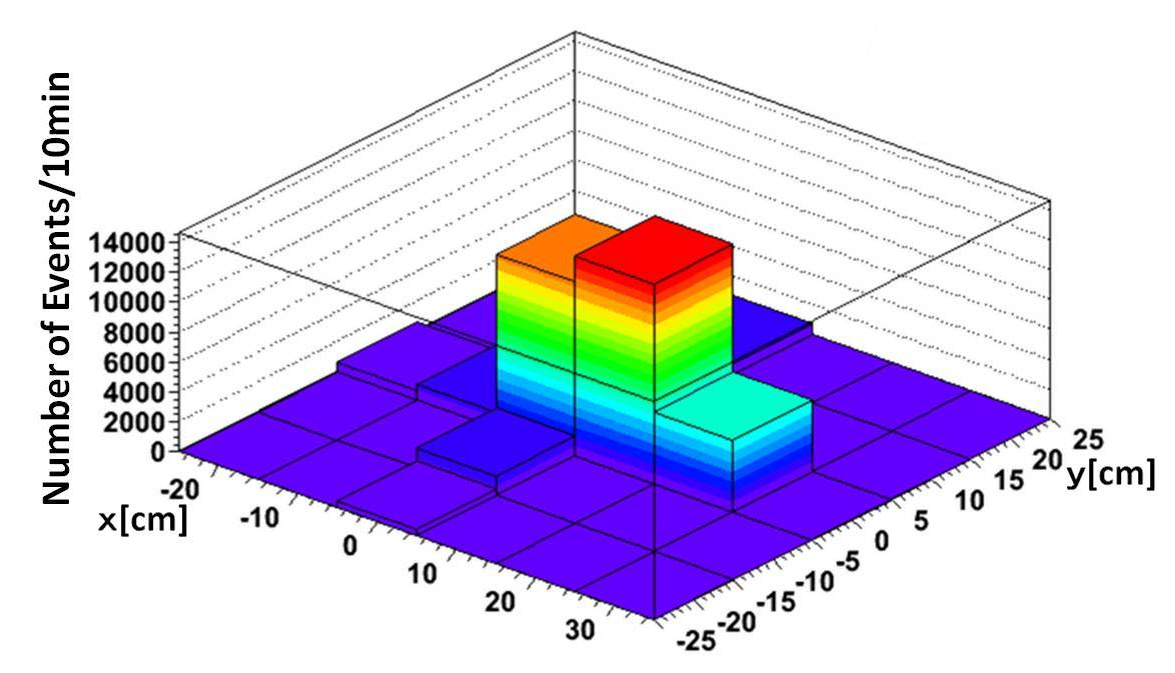
\includegraphics[width=11cm,clip]{./fig/BeamProfile3.eps}
    \caption{Beam profile on the front of 250LAr TPC}
    \label{beamprofile_250L}
   \end{figure}

